% !TEX root = main.tex

\section{Lecture 15:  Arbitrary Lagrangian--Eulerian scheme}
\begin{flushright}\textbf{[by Christelle Auguste]}\end{flushright}

{\color{red} Navid: I'm working on these notes.}

The Arbitrary Lagrangian--Eulerian (ALE) method combines the best features of Lagrangian and Eulerian representations. In Lagrangian simulations the mesh moves with the local velocity, in Eulerian  simulations the mesh is fixed in space and the fluid moves from one cell to another. The initial representation of the ALE method was described by \citet{1974JCoPh..14..227H}. There are two general methods of ALE in ocean models: quasi-Eulerian and quasi-Lagrangian algorithm (used by MOM6). This lecture focuses on the latter.

The added features of the ALE method provide the opportunity to increase the model time step (removal of the vertical Courant--Friedrichs--Lewy). The stability criterion known as Courant--Friedrichs--Lewy condition or CFL condition is:
\begin {align}
\mathrm{CFL}&=\Delta t <\frac{\Delta x}{2c}.
\end{align}
with the CFL number equal to :
\begin{equation}
C \equiv \frac{u \Delta t}{\Delta x}.
\end{equation}
The Courant number is a measure of how much information traverses $u$ a computational grid cell $\Delta x$ in a given time-step $\Delta t$.
The time step must be less than a certain time in many explicit time marching computer simulations, otherwise the simulation will produce incorrect results. CFL condition it is necessary to define correctly the time step simulation. The Courant number must be equal or smaller than 1, otherwise, the numerical viscosity would be negative.

{\color{red}[Navid: 1. Please punctuate equations.]}\\
{\color{red}[Navid: 2. The CFL is a non-dimensional number $u dt/dx$ and this number should be less than 1 or 0.5 for the simulation to be stable. Can you 1) fix your definition above and 2) provide a bit more details for what CFL is and why it should be less than one? (I mean 1-2 sentences...). If you need help let me know.]}\\

Consider
\begin{equation}
    \frac{\partial p}{\partial z} =- g \rho (Z, \delta^n, \sigma^n).
\end{equation}
with $n = \text{time level}$.

Now consider the Boussinesq hydrostatic equations for thickness:
 \begin{equation}
     \frac{\partial h}{\partial t} + \boldsymbol{\nabla}_\sigma \cdot(h \boldsymbol{U})+\Delta_\sigma (w^{\dot{\sigma }})=0.
 \end{equation}
 with $w^{\dot{\sigma }}$ equal to the Dia-surface velocity component.
 \begin{figure}[h!]
  \centering
  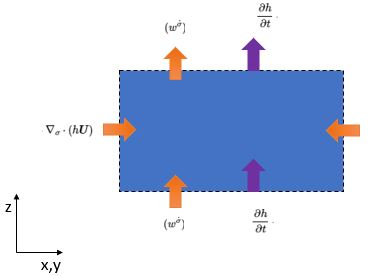
\includegraphics[width=3in]{lecture15_thicknessequation}
    \caption{Mapping of Thickness equation }
  \end{figure}

 \begin{equation}
     \frac{h^{n+1}-h^n}{\Delta t}= -\boldsymbol{\nabla}_\sigma(h\boldsymbol{U})- \Delta_\sigma (w^{\dot{\sigma }}).
 \end{equation}

 where ${\Delta_\sigma (w^{\dot{\sigma }}})$ is negligible, which gives:
  \begin{equation}
     h^\dagger=h^n-\Delta t \boldsymbol{\nabla}_\sigma(h\boldsymbol{U}^n)\label{L15:Regrid}.
 \end{equation}
 with $h^\dagger$ an incomplete version of $h^{n+1}$, the one we are looking for.
 
 We use the same process for $\boldsymbol{U}$ and we obtain:
 \begin{equation}
     \boldsymbol{U}^\dagger=\boldsymbol{U}^n-\Delta t (...).
 \end{equation}
 \\$h^\dagger$ and $\boldsymbol{U}^\dagger$ are  solutions to the shallow water equations.
 
 Concretely in the model we discretised with Lagrangian form at the beginning of the simulation, the second step in the algorithm is to regrid then to remap. 
 \\On Figure 15.1 are represented this steps used to time step the fluid state. The step regrid acts to reinitialize the vertical coordinate by locating the new vertical grid, the corresponding equation is Eq.~\eqref{L15:Regrid}: the new thickness is prescribed by the new grid. In this step the advection is no longer linked to CFL. The step remap acts to remap all variables from the old grid onto the new grid, and the corresponding equation for remap tracer is:
  \begin{equation}
     h^\dagger C^\dagger=h^nC^n+\Delta t \boldsymbol{\nabla}_\sigma(\boldsymbol{U}^nC^n)\label{L15:Remap}.
 \end{equation}
 %is it right for the last term?? was not written by Andy....
 
  \begin{figure}[h!]
  \centering
  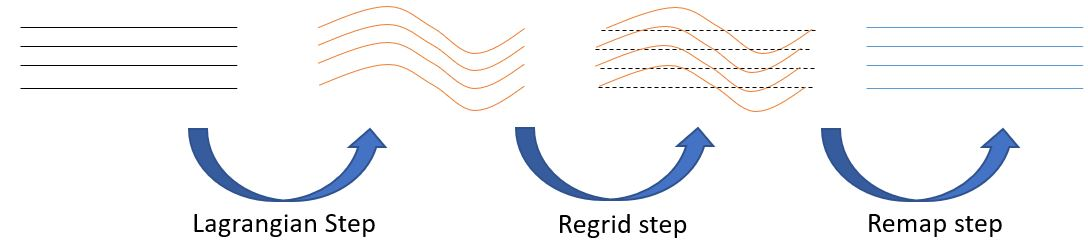
\includegraphics[width=5in]{figures/lecture15_stepsale.JPG}
  \caption{Steps for ALE algorithm. (Figure modified from \citet{Griffies2019}.) {\color{red}[Navid: Christelle, can you remove the red spell-checking underlines from the figure labels?] // Done}}
  \end{figure}

Example with internal waves, consider $\eta_k ^0$ 

when Z goes to infinity, when remapping instead of going back to the initial state we have:
 \begin{equation}
  \eta_{k}^{n+1} = \frac{(\eta_{k}^\dagger - \eta_{k}^0)\Delta t}{\tau}.
 \end{equation}
 with $\tau$ the time scale
 \\If the time step is fast, less than a day this step stay the same, and over a long term period come back to zero: the long term evolution of the ocean is not Lagrangian.
 
 
  Case of Adaptive grid:
  \begin{equation}
     \frac{\partial \eta_k}{\partial t} =- \boldsymbol{\nabla}_\sigma(\alpha_\sigma\frac{k\boldsymbol{\nabla}_\sigma \rho}{\sqrt{(\partial{z} \rho)^2+(\boldsymbol{\nabla}_\sigma \rho)^2}}+\alpha_\sigma K\boldsymbol{\nabla}_\sigma \eta_k) .
 \end{equation}
 %% don't know how to explain this equation!
  \begin{figure}[h!]
  \centering
  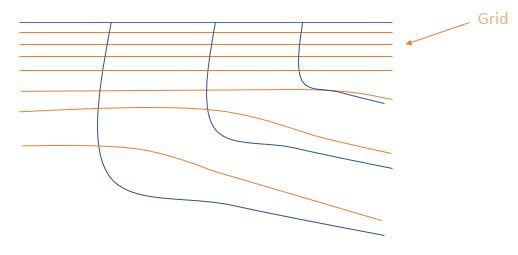
\includegraphics[width=5in]{figures/lecture15_adaptivegrid.JPG}
    \caption{Schematic adaptive grid.}
    \label{fig:lecture15_adaptivegrid}
    \end{figure}
  In this case the grid is following the isopycnal.
  
 In ocean models, mixing has two components : physical and numerical.The physical comes from advection by unresolved turbulence (diffusivity), and numerical from errors in the discretisation to solve the governing equations \citep{GIBSON201745}.Numerical mixing is also called spurious mixing, and we aim to minimise this term. ALE method can reduce spurious mixing by remapping to continuous isopycnal coordinates (Fig. \ref{fig:lecture15_adaptivegrid}).
 
